{ \setbeamercolor{background canvas}{bg=hl_bg}
  \setbeamercolor{normal text}{fg=hl_fg}
  \setbeamercolor{frametitle}{fg=hl_fg}
  \begin{frame}{What Have We been Talking About?}
    \usebeamercolor[fg]{normal text}
    
    \begin{tikzpicture}
      \tikzstyle{cnode} = [thick, ellipse, align=center, draw, inner sep = 6pt]
      \tikzstyle{nnode} = [thick, rectangle, rounded corners = 2pt,minimum size = 0.8cm,draw,inner sep = 6pt]
      \node[nnode] (kl) at (0,0) {KL-divergence};
      \node[nnode, right= 5cm of kl] (freeEnergy) {\begin{tabular}{c}Free energy $F_V(q(\bm{x}_U|\bm{x}_O))$ \\ (Variational/Gibbs)\end{tabular}};
      \node[nnode, below= of freeEnergy] (elbo) {\begin{tabular}{c}Evidence lower\\ bound $F(q(\bm{x}_U|\bm{x}_O))$ (ELBO)\end{tabular}};
      \node[nnode, below= of kl] (q-fun) {\begin{tabular}{c}Q-function\\ in EM\end{tabular}};
      \node[nnode, below right= of q-fun] (llk) {log-likelihood $\log{p(\bm{x}_O;\bm{\theta})}$};
      \draw[black, ->] (kl) --node [text width=5cm, black, midway, above]{\tiny
        \begin{tabular}{c}
          Diff. by a sub-partition func. \\
          $F_V(q(\bm{x}_U|\bm{x}_O)) = \mathrm{KL}(q(\bm{x}_U|\bm{x}_O) || p(\bm{x}_U|\bm{x}_O; \bm{\theta})) $ \\
          $- \log{Z(\bm{x}_O; \bm{\theta})}$
        \end{tabular}}
      (freeEnergy);
      \draw[black, ->] (freeEnergy) --node [text width=3cm, black, midway, left]{\tiny
        \begin{tabular}{c}
          Negative \\
          $F(q(\bm{x}_U|\bm{x}_O)) = -F_V(q(\bm{x}_U|\bm{x}_O))- \underbrace{\log{Z(\bm{\theta})}}_{\text{0 in DAGs}}$
        \end{tabular}}
      (elbo);

      \draw[black, ->] (kl) --node [text width=3cm, black, midway, left]{\tiny
        \begin{tabular}{c}
          $-\mathrm{KL}(q(\bm{x}_U|\bm{x}_O) || p(\bm{x}_U,\bm{x}_O; \bm{\theta})) $
        \end{tabular}}
      (elbo);

      \draw[black, ->] (elbo) --node [text width=3cm, black, midway, above]{\tiny
        \begin{tabular}{c}
          Diff. by an Entropy term\\
          $F(q(\bm{x}_U|\bm{x}_O))= \Qq + H({q(\bm{x}_U|\bm{x}_O)})$
        \end{tabular}}
      (q-fun);

      \draw[black, ->] (elbo) --node [text width=3cm, black, midway, above]{\tiny
        Below
      }
      (llk);
      \draw[black, ->] (q-fun) --node [text width=3cm, black, midway, right]{\tiny
        Below
      }
      (llk);
      
    \end{tikzpicture}
    \only<2->{
      \begin{textblock}{5}(6,6)
        \begin{tikzpicture}[scale=1.2,auto,rotate=-5,transform shape]
          \tikzstyle{cnode} = [fill=blue!20,thick, ellipse, align=center, draw, inner sep = 6pt]
          \node [cnode, text=black] (question) at (0, 0) {\begin{tabular}{c}What if lklh. \\is not tractable?\end{tabular}};
          
        \end{tikzpicture}
      \end{textblock}
    }
    % \let\thefootnote\relax\footnotetext{\tiny
    % \vskip -0.2cm
    % A bit notation abuse, $\bm{x}_U$ corresponds to unobserved variable $\bm{z}$.
    % }
    
  \end{frame}
}

{ \setbeamercolor{background canvas}{bg=hl_bg}
  \setbeamercolor{normal text}{fg=hl_fg}
  \setbeamercolor{frametitle}{fg=hl_fg}
  \begin{frame}
    \usebeamercolor[fg]{normal text}
    \begin{center}
      {
        \begin{tikzpicture}
          \tikzstyle{cnode} = [thick, draw=white, ellipse, inner sep = 2pt,  align=center]
          \tikzstyle{fnode} = [thick, draw=white, ellipse, inner sep = 10pt,  align=center]
          \tikzstyle{rnode} = [thick, rectangle, inner sep = 1.5pt,  align=left]
          \node[rnode] (inf) at (-2, 0) {\large Inference};
          \node[rnode, below = 0.6cm of inf.west, anchor=west] (abp) {$\bullet$ {$\alpha$-BP}};
          \node[rnode, below = 1.2cm of inf.west, anchor=west] (renn) {$\bullet$ RENN};
          \node[cnode, fit=(abp)(inf)(renn)] (infn) {};
          
          \node[rnode, right = 3 of inf] (lern) {\large Learning};
          \node[rnode, below = 0.4 of lern.west, anchor=west] (genmm) {$\bullet$ GenMM};
          \node[rnode, below = 0.8 of lern.west, anchor=west] (genhmm) {{$\bullet$} GenHMM};
          \node[rnode, below = 1.2 of lern.west, anchor=west] (lfree) {\textbf{{$\bullet$} EOTGM}};
          \node[cnode, fit=(lern)(genmm)(genhmm)(lfree)] (learn) {};
          \node[rnode, draw=green, fit=(lfree)] () {};

          \node[fnode, fit=(infn)(lern)] (box) {};

          
          \node[below right = 0.5 and -0.5 of infn] {{Probabilistic} Graphical Model};
          \draw[->,line width=0.2mm] (infn) to[out=15, in=165] (learn);
          \draw[->,line width=0.2mm] (learn) to[out=195, in=-15] (infn);
        \end{tikzpicture}
      }
    \end{center}
    
  \end{frame}
}

\begin{frame}{Where is the learning info. from?}
  \begin{tikzpicture}
    \tikzstyle{enode} = [thick, draw, circle, inner sep = 4pt,  align=center]
    \tikzstyle{elnode} = [thick, draw, ellipse, inner sep = 1pt,  align=center]
    \tikzstyle{nnode} = [thick, rectangle, rounded corners = 2pt,draw,inner sep = 4pt]
    \node[enode] (z) at (-4,0) {$\bm{Z}$};
    \node[enode, right=2cm of z] (x) {$\bm{X}$};
    \node[elnode] (emp) [right= 6.5cm of x] {Empirical \\samples};
    
    \draw[->] (z) -- node[nnode,fill=white] {$\bm{g}$} (x);
    \draw[<->] (x) -- node[draw, rounded corners = 2pt, fill=blue!30, align=center] (trckmetric) {
      \begin{minipage}{0.45\textwidth}
        How different they are
        \begin{itemize}[label=\textbullet]
        \item likelihood
        \item Evidence lower bound, free energy 
        \item KL-divergence, $\alpha$-divergence
        \end{itemize}
      \end{minipage}} (emp);
    \node[fill=white!30, below= of trckmetric, align=center] (ot) {
      \begin{minipage}{0.6\textwidth}
        Optimal transport (OT): moving mass from a dist. to another
        \begin{equation*}
          T(p^{\ast},p)=\min_{ \pi \in \Pi(p^{\ast},p)} \dotp{\underbrace{\pi}_{\text{marginalize to $p^{\ast},p$}}}{\underbrace{\bm{M}}_{\text{\begin{tabular}{c}cost matrix\\ sample difference \end{tabular}}}},
        \end{equation*}
        Key attributes:
        \begin{itemize}[label=\textbullet]
        \item Doesnot require tractible lklh.
        \item Learning gradient info. from sample comparison
        \item High complexity, each evaluation is sovling an optimization problem
        \end{itemize}
      \end{minipage}
    };
    \draw[->] (trckmetric) -- node[black, midway, right] {add-on} (ot);

  \end{tikzpicture}
  \only<2>{
    \begin{textblock}{5}(2,4.3)
      \begin{tikzpicture}
        \node[rounded corners = 4pt, rectangle, inner sep = 4pt, fill=gray!20, align=center, text width=10cm, label=below:{A toy example}] (ot_kl) at (0,0)
        {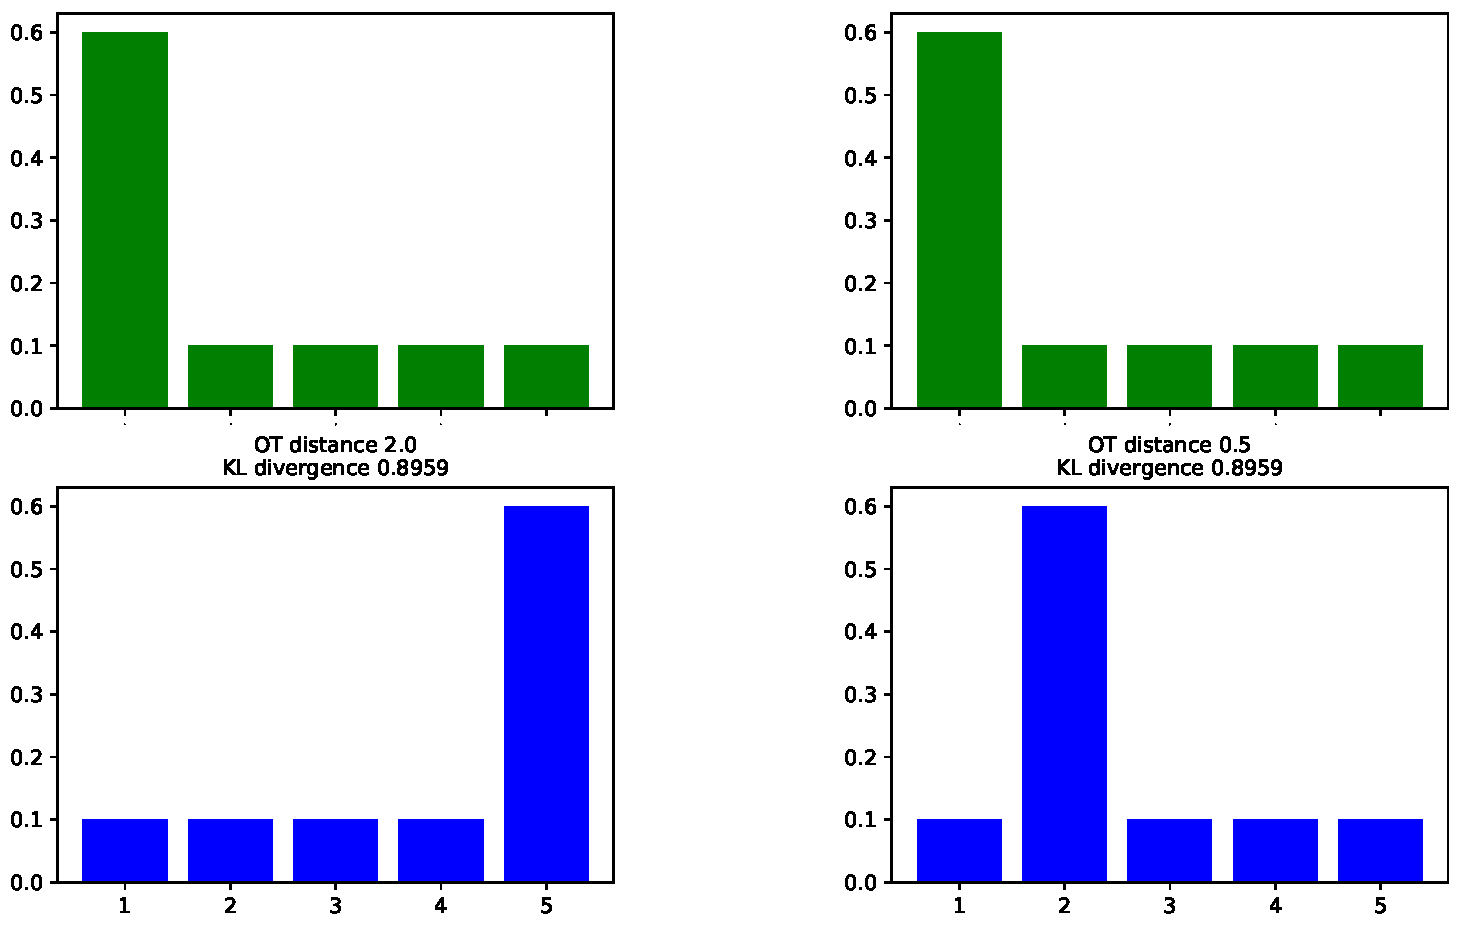
\includegraphics[width=1\linewidth]{images/ot_kl.pdf}};
      \end{tikzpicture}
    \end{textblock}
  }
\end{frame}


\begin{frame}{EOTGM: EOT based Generative Model}
  \begin{tikzpicture}
    \tikzstyle{enode}=[thick, draw, circle, inner sep = 8pt,  align=center]
    \tikzstyle{elnode}=[thick, draw, rectangle, rounded corners = 2pt, inner sep = 4pt, align=center]
    \tikzstyle{nnode} = [thick, rectangle, rounded corners = 2pt,minimum size = 4.8cm,draw,inner sep = 2pt]
    \node[elnode] (ot) at (-1,0) {OT $\min\;T(p^{\ast},p)$};
    % \node[nnode] at (0,1) {$T(P,Q) = \min_{\Gamma\in\Pp(P,Q) }\EE_{(X,Y)\sim \Gamma}\left[ c(X,Y) \right]$};
    \node[elnode] (wgan) at (6,0) {\begin{tabular}{c}WGAN, Arjovsky, et al\\ {\tiny Wasserstein Generative Adversarial Network} \\ {\tiny An adversarial game} \\ {\tiny \textit{1-Lipschitz function family}}\end{tabular}};
    \node[elnode] (eot) at (3,-2) {\begin{tabular}{c} EOTGM \\ {\tiny NN generator + Sinkhorn solver} \\ {\tiny Applicable to implicit \& explicit models} \end{tabular}};
    \draw[->] (ot) -- node[midway,above] {\tiny Kantorovich duality} (wgan);
    \draw[->] (ot) -- node[midway,right] {\tiny Entropy regularization} (eot);
    \node[text width=4cm] [right=-0.1cm of eot] {\begin{equation*} \min_{p} \underbrace{\min_{\pi\in\Pp(p^{\ast},p) } \dotp{\pi}{\bm{M}} - \la H(\pi)}_{W(p^{\ast}, p)}
      \end{equation*}};   
  \end{tikzpicture}
  Alternatively scale the rows \& columns of matrix $e^{-\bm{M}/\lambda}$ (Sinkhorn \& Knopp) gives 'soft' solution
  \begin{itemize}[label=\textbullet]
  \item joint distribution $\pi^{\ast}$
  \item subgradient $\beta^{\ast}$
  \end{itemize}
  which provides the gradient information for adjusting $\bm{g}$.
  \only<2>{
    \begin{textblock}{5}(2,4.3)
      \begin{tikzpicture}
        
        \begin{scope}[scale=1.6, local bounding box=algo]
          % Graphic for TeX using PGF
% Title: /home/dong/Documents/phd_research/my_papers/entropy-wgan/poster/figs/alo_flow.dia
% Creator: Dia v0.97.3
% CreationDate: Wed Apr 24 18:01:40 2019
% For: dong
% \usepackage{tikz}
% The following commands are not supported in PSTricks at present
% We define them conditionally, so when they are implemented,
% this pgf file will use them.
\ifx\du\undefined
  \newlength{\du}
\fi
\setlength{\du}{5\unitlength}
\pgftransformxscale{1.000000}
\pgftransformyscale{-1.000000}
\definecolor{dialinecolor}{rgb}{0.000000, 0.000000, 0.000000}
\pgfsetstrokecolor{dialinecolor}
\definecolor{dialinecolor}{rgb}{1.000000, 1.000000, 1.000000}
\pgfsetfillcolor{dialinecolor}
\pgfsetlinewidth{0.100000\du}
\pgfsetdash{}{0pt}
\pgfsetdash{}{0pt}
\pgfsetbuttcap
{
\definecolor{dialinecolor}{rgb}{0.000000, 0.000000, 0.000000}
\pgfsetfillcolor{dialinecolor}
% was here!!!
\definecolor{dialinecolor}{rgb}{0.000000, 0.000000, 0.000000}
\pgfsetstrokecolor{dialinecolor}
\draw (18.524007\du,0.865483\du)--(18.528518\du,3.644891\du);
}
\pgfsetlinewidth{0.100000\du}
\pgfsetdash{}{0pt}
\pgfsetdash{}{0pt}
\pgfsetbuttcap
{
\definecolor{dialinecolor}{rgb}{0.000000, 0.000000, 0.000000}
\pgfsetfillcolor{dialinecolor}
% was here!!!
\definecolor{dialinecolor}{rgb}{0.000000, 0.000000, 0.000000}
\pgfsetstrokecolor{dialinecolor}
\draw (18.500105\du,3.590367\du)--(27.515393\du,3.588352\du);
}
\pgfsetlinewidth{0.100000\du}
\pgfsetdash{}{0pt}
\pgfsetdash{}{0pt}
\pgfsetbuttcap
{
\definecolor{dialinecolor}{rgb}{0.000000, 0.000000, 0.000000}
\pgfsetfillcolor{dialinecolor}
% was here!!!
\definecolor{dialinecolor}{rgb}{0.000000, 0.000000, 0.000000}
\pgfsetstrokecolor{dialinecolor}
\draw (9.531143\du,3.591676\du)--(18.546431\du,3.589661\du);
}
\pgfsetlinewidth{0.100000\du}
\pgfsetdash{}{0pt}
\pgfsetdash{}{0pt}
\pgfsetbuttcap
{
\definecolor{dialinecolor}{rgb}{0.000000, 0.000000, 0.000000}
\pgfsetfillcolor{dialinecolor}
% was here!!!
\pgfsetarrowsend{latex}
\definecolor{dialinecolor}{rgb}{0.000000, 0.000000, 0.000000}
\pgfsetstrokecolor{dialinecolor}
\draw (9.554590\du,3.555355\du)--(9.545014\du,6.552207\du);
}
\pgfsetlinewidth{0.100000\du}
\pgfsetdash{}{0pt}
\pgfsetdash{}{0pt}formu
\pgfsetbuttcap
{
\definecolor{dialinecolor}{rgb}{0.000000, 0.000000, 0.000000}
\pgfsetfillcolor{dialinecolor}
% was here!!!
\pgfsetarrowsend{latex}
\definecolor{dialinecolor}{rgb}{0.000000, 0.000000, 0.000000}
\pgfsetstrokecolor{dialinecolor}
\draw (27.515539\du,3.579062\du)--(27.518490\du,6.615272\du);
}
% setfont left to latex
\definecolor{dialinecolor}{rgb}{0.000000, 0.000000, 0.000000}
\pgfsetstrokecolor{dialinecolor}
\node[anchor=west] at (18.801352\du,2.255187\du){\tiny Explicity model?};
% setfont left to latex
\definecolor{dialinecolor}{rgb}{0.000000, 0.000000, 0.000000}
\pgfsetstrokecolor{dialinecolor}
\node[anchor=west] at (12.404325\du,3.043961\du){Yes};
% setfont left to latex
\definecolor{dialinecolor}{rgb}{0.000000, 0.000000, 0.000000}
\pgfsetstrokecolor{dialinecolor}
\node[anchor=west] at (25.516919\du,3.045657\du){No};
\pgfsetlinewidth{0.100000\du}
\pgfsetdash{}{0pt}
\pgfsetdash{}{0pt}
\pgfsetmiterjoin
\definecolor{dialinecolor}{rgb}{0.000000, 0.000000, 0.000000}
\pgfsetstrokecolor{dialinecolor}
\draw (6.132662\du,6.958798\du)--(6.132662\du,13.481742\du)--(17.882368\du,13.481742\du)--(17.882368\du,6.958798\du)--cycle;
\pgfsetlinewidth{0.100000\du}
\pgfsetdash{}{0pt}
\pgfsetdash{}{0pt}
\pgfsetmiterjoin
\definecolor{dialinecolor}{rgb}{0.000000, 0.000000, 0.000000}
\pgfsetstrokecolor{dialinecolor}
\draw (18.629924\du,6.913963\du)--(18.629924\du,13.436908\du)--(30.379629\du,13.436908\du)--(30.379629\du,6.913963\du)--cycle;
% setfont left to latex
\definecolor{dialinecolor}{rgb}{0.000000, 0.000000, 0.000000}
\pgfsetstrokecolor{dialinecolor}
\node[anchor=west] at (5.856351\du,10.251070\du){\tiny {\vbox{
  \begin{itemize}[label=\textbullet]
  \item Gradient chain rule
  \item Direct optimization
    \item[] w.r.t. model parameters
  \end{itemize}}}};
% setfont left to atex
\definecolor{dialinecolor}{rgb}{0.000000, 0.000000, 0.000000}
\pgfsetstrokecolor{dialinecolor}
\node[anchor=west] at (18.52029\du,10.254778\du){\tiny {\vbox{
      \begin{itemize}[label=\textbullet]
        \item Richer choice of $\bm{g}$
  \item Formulate loss by $\pi^{\ast}_{\lambda}$
  \item Error back-propagation
    \item[] by auto gradient tools
  \end{itemize}}}};
\pgfsetlinewidth{0.100000\du}
\pgfsetdash{}{0pt}
\pgfsetdash{}{0pt}
\pgfsetbuttcap
\pgfsetmiterjoin
\pgfsetlinewidth{0.100000\du}
\pgfsetbuttcap
\pgfsetmiterjoin
\pgfsetdash{}{0pt}
\definecolor{dialinecolor}{rgb}{0.000000, 0.000000, 0.000000}
\pgfsetstrokecolor{dialinecolor}
\draw (15.723295\du,-3.076184\du)--(16.205111\du,-6.930706\du)--(20.541447\du,-8.857967\du)--(24.877784\du,-6.930706\du)--(25.359599\du,-3.076184\du)--(22.950523\du,0.296522\du)--(18.132371\du,0.296522\du)--cycle;
\pgfsetlinewidth{0.010000\du}
\pgfsetbuttcap
\pgfsetmiterjoin
\pgfsetdash{}{0pt}
\definecolor{dialinecolor}{rgb}{0.000000, 0.000000, 0.000000}
\pgfsetstrokecolor{dialinecolor}
\draw (15.723295\du,-3.076184\du)--(16.205111\du,-6.930706\du)--(20.541447\du,-8.857967\du)--(24.877784\du,-6.930706\du)--(25.359599\du,-3.076184\du)--(22.950523\du,0.296522\du)--(18.132371\du,0.296522\du)--cycle;
\pgfsetlinewidth{0.100000\du}
\pgfsetdash{}{0pt}
\pgfsetdash{}{0pt}
\pgfsetbuttcap
{
\definecolor{dialinecolor}{rgb}{0.000000, 0.000000, 0.000000}
\pgfsetfillcolor{dialinecolor}
% was here!!!
\pgfsetarrowsstart{latex}
\definecolor{dialinecolor}{rgb}{0.000000, 0.000000, 0.000000}
\pgfsetstrokecolor{dialinecolor}
\draw (14.704266\du,-9.125968\du)--(10.750000\du,-0.302492\du);
}
\pgfsetlinewidth{0.100000\du}
\pgfsetdash{}{0pt}
\pgfsetdash{}{0pt}
\pgfsetmiterjoin
\pgfsetbuttcap
{
\definecolor{dialinecolor}{rgb}{0.000000, 0.000000, 0.000000}
\pgfsetfillcolor{dialinecolor}
% was here!!!
\pgfsetarrowsstart{latex}
\definecolor{dialinecolor}{rgb}{0.000000, 0.000000, 0.000000}
\pgfsetstrokecolor{dialinecolor}
\pgfpathmoveto{\pgfpoint{18.132371\du}{0.296522\du}}
\pgfpathcurveto{\pgfpoint{18.682371\du}{-2.653478\du}}{\pgfpoint{20.600968\du}{-2.060704\du}}{\pgfpoint{21.200968\du}{-4.360704\du}}
\pgfusepath{stroke}
}
\pgfsetlinewidth{0.100000\du}
\pgfsetdash{{1.000000\du}{1.000000\du}}{0\du}
\pgfsetdash{{1.000000\du}{1.000000\du}}{0\du}
\pgfsetbuttcap
{
\definecolor{dialinecolor}{rgb}{0.000000, 0.000000, 0.000000}
\pgfsetfillcolor{dialinecolor}
% was here!!!
\definecolor{dialinecolor}{rgb}{0.000000, 0.000000, 0.000000}
\pgfsetstrokecolor{dialinecolor}
\draw (11.839663\du,-2.816111\du)--(18.080386\du,0.347759\du);
}
\pgfsetlinewidth{0.100000\du}
\pgfsetdash{}{0pt}
\pgfsetdash{}{0pt}
\pgfsetbuttcap
{
\definecolor{dialinecolor}{rgb}{0.000000, 0.000000, 0.000000}
\pgfsetfillcolor{dialinecolor}
% was here!!!
\definecolor{dialinecolor}{rgb}{0.000000, 0.000000, 0.000000}
\pgfsetstrokecolor{dialinecolor}
\draw (12.356671\du,-2.597719\du)--(12.670233\du,-3.241992\du);
}
\pgfsetlinewidth{0.100000\du}
\pgfsetdash{}{0pt}
\pgfsetdash{}{0pt}
\pgfsetbuttcap
{
\definecolor{dialinecolor}{rgb}{0.000000, 0.000000, 0.000000}
\pgfsetfillcolor{dialinecolor}
% was here!!!
\definecolor{dialinecolor}{rgb}{0.000000, 0.000000, 0.000000}
\pgfsetstrokecolor{dialinecolor}
\draw (12.676482\du,-3.210742\du)--(12.096348\du,-3.498168\du);
}
% setfont left to latex
\definecolor{dialinecolor}{rgb}{0.000000, 0.000000, 0.000000}
\pgfsetstrokecolor{dialinecolor}
\node[anchor=west] at (18.030166\du,-5.041491\du){$p^{\ast}\cdot p^{\intercal}$, $\lambda \rightarrow \infty$};
% setfont left to latex
\definecolor{dialinecolor}{rgb}{0.000000, 0.000000, 0.000000}
\pgfsetstrokecolor{dialinecolor}
\node[anchor=west] at (12.022945\du,-7.745138\du){$\pd{W}{\theta}$};
\pgfsetlinewidth{0.100000\du}
\pgfsetdash{}{0pt}
\pgfsetdash{}{0pt}
\pgfsetbuttcap
\pgfsetmiterjoin
\pgfsetlinewidth{0.100000\du}
\pgfsetbuttcap
\pgfsetmiterjoin
\pgfsetdash{}{0pt}
\definecolor{dialinecolor}{rgb}{0.000000, 0.000000, 0.000000}
\pgfsetfillcolor{dialinecolor}
\pgfpathellipse{\pgfpoint{18.464159\du}{-1.026639\du}}{\pgfpoint{0.159762\du}{0\du}}{\pgfpoint{0\du}{0.159762\du}}
\pgfusepath{fill}
\definecolor{dialinecolor}{rgb}{0.000000, 0.000000, 0.000000}
\pgfsetstrokecolor{dialinecolor}
\pgfpathellipse{\pgfpoint{18.464159\du}{-1.026639\du}}{\pgfpoint{0.159762\du}{0\du}}{\pgfpoint{0\du}{0.159762\du}}
\pgfusepath{stroke}
\pgfsetbuttcap
\pgfsetmiterjoin
\pgfsetdash{}{0pt}
\definecolor{dialinecolor}{rgb}{0.000000, 0.000000, 0.000000}
\pgfsetstrokecolor{dialinecolor}
\pgfpathellipse{\pgfpoint{18.464159\du}{-1.026639\du}}{\pgfpoint{0.159762\du}{0\du}}{\pgfpoint{0\du}{0.159762\du}}
\pgfusepath{stroke}
% setfont left to latex
\definecolor{dialinecolor}{rgb}{0.000000, 0.000000, 0.000000}
\pgfsetstrokecolor{dialinecolor}
\node[anchor=west] at (18.985501\du,-0.965533\du){$\pi^{\ast}_{\lambda}$};



        \end{scope}
        \begin{scope}[on background layer]
          \node[rounded corners = 4pt, rectangle, inner sep = 4pt, fill=gray!20, align=center, text width=10cm, label=below:{}, fit=(algo)] () {};
        \end{scope}
        
      \end{tikzpicture}
    \end{textblock}
  }

  \let\thefootnote\relax\footnotetext{\tiny
    Marco Cuturi. Sinkhorn distances: Lightspeed computation of optimal transport}
\end{frame}

\begin{frame}[label=current]{EOTGM and EOTGAN}
  EOTGM\\
  \begin{tikzpicture}
    \tikzstyle{enode} = [draw, circle, inner sep = 4pt,  align=center]
    \tikzstyle{nnode} = [rectangle, rounded corners = 2pt,draw,inner sep = 4pt]
    \tikzstyle{ecnode} = [draw, ellipse, inner sep = 4pt,  align=center]

    \begin{scope}[scale=0.7, every node/.append style={transform shape}]
      \node[enode] (z) at (-4,0) {$\bm{Z}$};
      \node[enode, right=2cm of z] (x) {$\bm{X}$};
      \node[enode, below= of x] (hx) {$\hat{\bm{X}}$};
      \node[ecnode, below= of z] (data) {Dataset};

      \draw[->] (z) -- node[nnode,fill=white] {$\bm{g}$} (x);
      \draw[->] (data) -- (hx);
      % \node[nnode, fit=(x) (hx) ($(hx.south west) + (-0.2, -0.2)$), label={below:{\tiny Input}}, dashed] (inPair) {};

      \draw[green, ->] ($(z.north) + (0,0.6)$) -- node [black, midway, above] {\tiny generated v.s. empirical sample comparison} ($(z.north) + (5,0.6)$);
      \draw[green, <-] ($(z.north) + (0,-3.6)$) -- node [black, midway, below] {\tiny subgradient info.} ($(z.north) + (5,-3.6)$);
    \end{scope}
    \node[nnode, fit=(x) (hx), label={below:{\tiny Input}}, dashed] (inPair) {};  
    \node[nnode, rotate=-90, inner sep = 8pt, fill=gray!15] (rowScale) at (1,-0.6) {\tiny ~~Row Scale~~~~};
    \node[nnode, rotate=-90, inner sep = 8pt, fill=gray!5] (colScale) at (3,-0.6) {\tiny Column Scale};

    \draw[->] (inPair) to (rowScale);
    \only<1>{
      \draw [-{Straight Barb[left]}] ($(rowScale.north) + (0, 0.1) $) to ($(colScale.south) +(0,0.1)$);
      \draw [-{Straight Barb[left]}] (colScale) -- node[black, midway, below] {\tiny iterative} (rowScale) ;
    }
    \only<2>{
      \node[nnode, rotate=-90, inner sep = 8pt, fill=gray!15] (rowScale1) at (5,-0.6) {\tiny ~~Row Scale~~~~};
      \node[nnode, rotate=-90, inner sep = 8pt, fill=gray!5] (colScale1) at (7,-0.6) {\tiny Column Scale};
      
      \foreach \x in {-0.5, -.25, 0, 0.25, 0.5}{
        \draw [->] ($(rowScale.north) + (0,\x)$) -- ($(colScale.south) +(0,\x)$);
      }
      \foreach \x in {-0.5, -.25, 0, 0.25, 0.5}{
        \draw [->] ($(rowScale1.north) + (0,\x)$) -- ($(colScale1.south) +(0,\x)$);
      }
      \draw [dashed] ($(colScale.north) + (0,0)$) -- node[black, fill=white] {......} ($(rowScale1.south) +(0,0)$);
      % under brace
      \draw [thick, decoration={ brace, mirror, raise=0.5cm }, decorate ] (rowScale.east) -- (colScale1.east) 
      node [pos=0.5,anchor=north,yshift=-0.55cm] {\tiny Unrolled concatenated feed-forward neural network}; 
    }
  \end{tikzpicture}

  
  EOTGAN: learn implicit distribution with feature mapping\\
  
  \begin{tikzpicture}
    \tikzstyle{ecnode} = [draw, ellipse, inner sep = 4pt,  align=center]
    \tikzstyle{enode} = [draw, circle, inner sep = 4pt,  align=center]
    \tikzstyle{nnode} = [rectangle, rounded corners = 2pt,draw,inner sep = 4pt]

    \begin{scope}[scale=0.85, every node/.append style={transform shape}]
      \node[enode] (z) at (-4,0) {$\bm{Z}$};
% \node[enode, right=2cm of z] (x) {$\bm{X}$};
% \node[nnode, right=2cm of x] (fx) {};
\node[nnode, above right=-0.5cm and 3cm of z, minimum height=2cm, label={below:{\tiny Feature mapping}}] (f1) {$\bm{f}$};
\node[nnode, right= of z] (g) {$\bm{g}$};
\draw[->] (z) -- (g);
\draw[->] (g) -- ($(f1.west) + (0,-0.6)$);


\node[ecnode, above= of g] (dt) {Dataset};
\draw[->] ($(dt.east) + (0, 0)$) -- ($(f1.west) + (0,0.6)$);
\draw[->] ($(dt.south) + (0, 0)$) -- ($(f1.west) + (0,0.2)$);

\node[ecnode, right= 3cm of f1] (gan) {\begin{tabular}{c} EOT based triplet loss \\ offer grad. for:\\ generator $\bm{g}$ \\ feature mapping $\bm{f}$\end{tabular}};
\draw[->] ($(f1.east) + (0,0.4)$) -- (gan.175) node[black, midway, above=0.51cm] (gf) {\tiny comparison gives grad. for $\bm{f}$};
\draw[->] ($(f1.east) + (0,0)$) -- (gan.180) ;
\draw[->] ($(f1.east) + (0,-0.4)$) -- (gan.185) node[black, midway, below=0.45cm] (gg) {\tiny comparison gives grad. for $\bm{g}$};

\node[ecnode, draw=blue,dashed,thin, minimum height=0.8cm] (gfan) at ($(f1.east) + (0.5,0.25)$) {};
\node[ecnode, draw=blue,dashed,thin, minimum height=0.8cm] (ggan) at ($(gan.185) + (-0.5,0)$) {};

\draw[blue] (gfan) -- (gf);
\draw[blue] (ggan) -- (gf);

\draw[blue] (ggan) -- (gg);

%%% Local Variables:
%%% mode: latex
%%% TeX-master: "../ppgm_slide"
%%% End:

    \end{scope}

  \end{tikzpicture}
  
\end{frame}

\graphicspath{{../source/chapter8/}}

\begin{frame}{Numerical}
  \begin{columns}
    \column{0.5\textwidth}
    \vskip 0.5cm
    {\tiny $\bm{\rightarrow}$ Toy distribution learning (target at $4$-mixture Gaussians) using EOTGM. Real samples (red '+') and contour
      (red curve), versus generated samples (blue 'o') and contour (blue curve) by $\bm{g}$.
      \vskip 0.2cm
      $\bm{\downarrow}$
      Comparison of IS and FID (on MNIST) versus mixing ratio r.
    }
    \column{0.4\textwidth}
    
    \begin{figure}
      \centering
      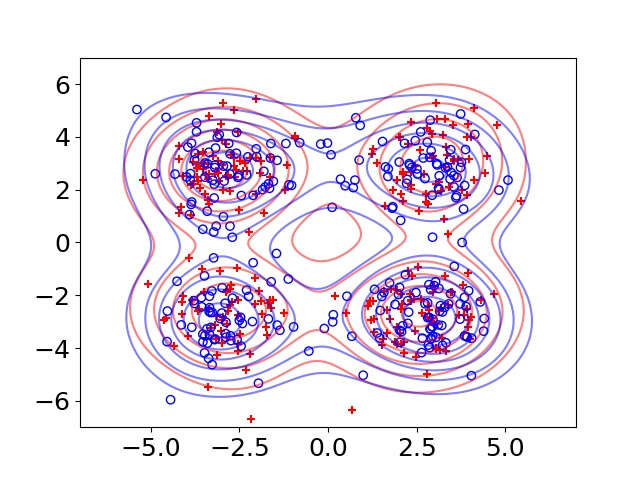
\includegraphics[width=1\linewidth]{images/toy/gauss4/frame8.jpg}
    \end{figure}
  \end{columns}
  \vskip -0.4cm
  \begin{figure}[!ht]
    \captionsetup[subfigure]{justification=centering}

    \begin{subfigure}[b]{0.44\textwidth}
      \centering
      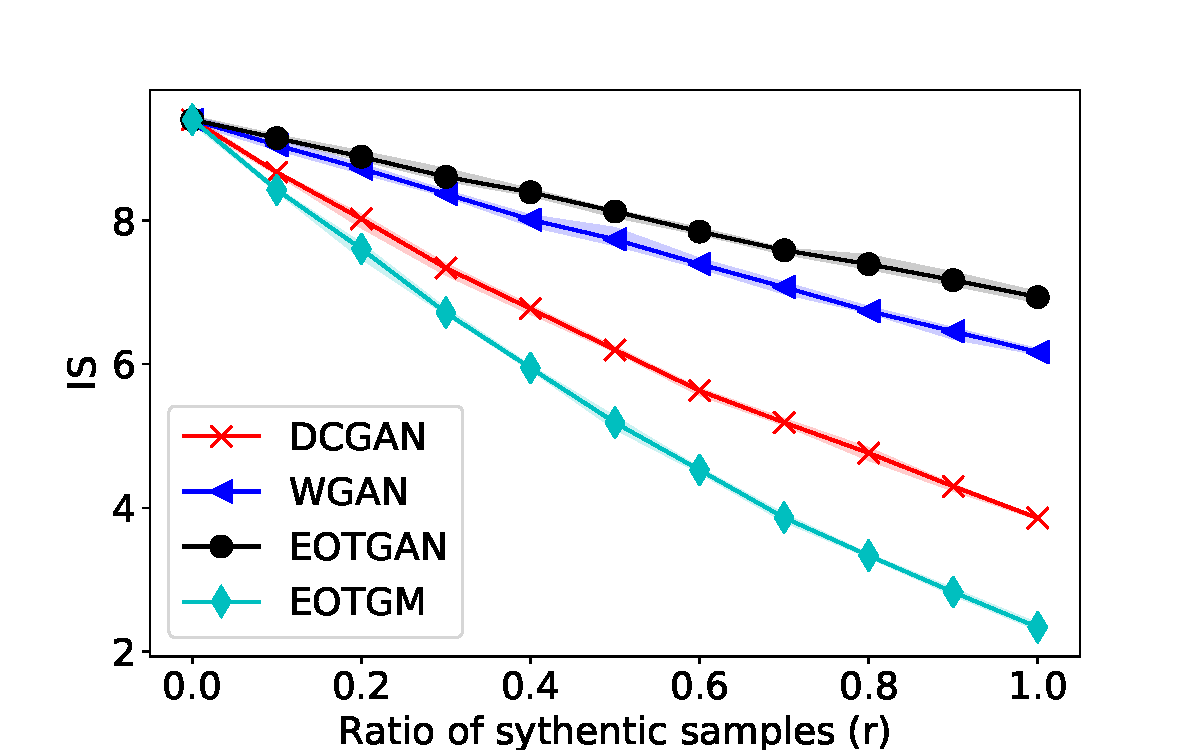
\includegraphics[width=1.1\linewidth]{images/mnist/tra_score/IS_29.pdf}\vspace{-3pt}
      % \caption{}
    \end{subfigure}
    \vspace{20pt}  
    \begin{subfigure}[b]{0.44\textwidth}
      \centering
      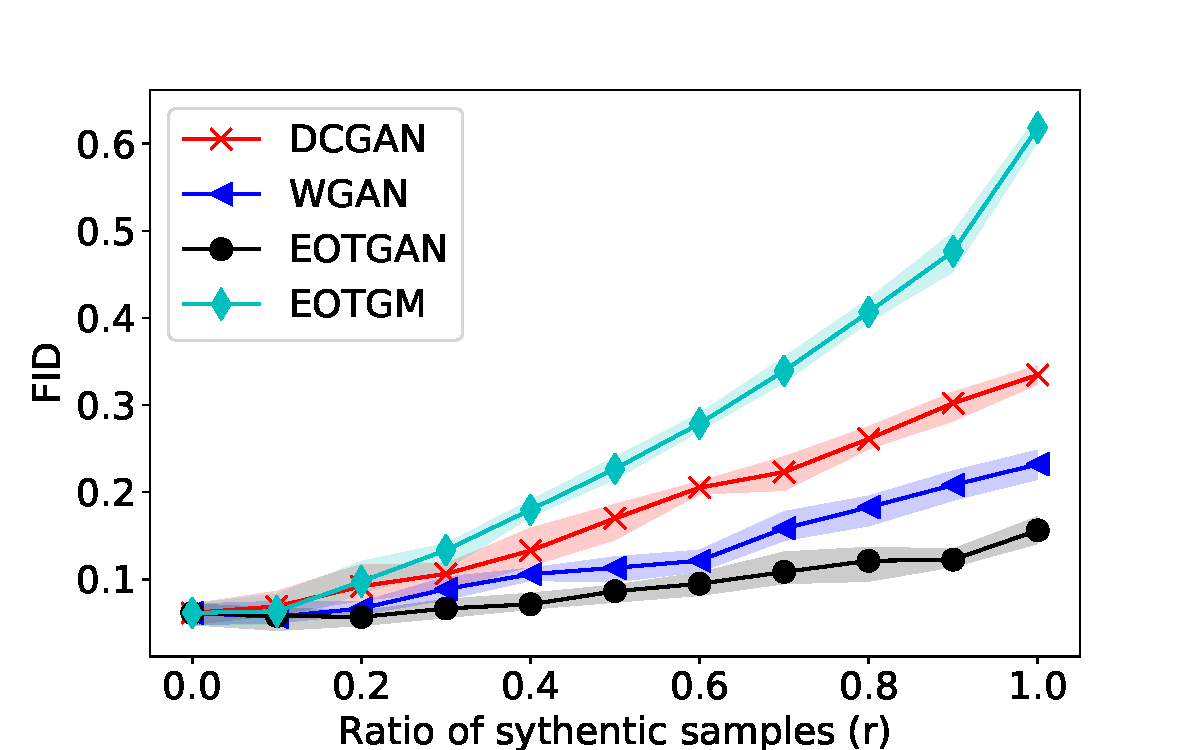
\includegraphics[width=1.1\linewidth]{images/mnist/tra_score/FID_29.pdf}\vspace{-3pt}
      % \caption{}
      
    \end{subfigure}
    % \vspace{-15pt}
    \captionsetup{labelformat=empty,justification=centering}
    \caption{Comparison of IS and FID (on MNIST) versus mixing ratio $r$. % (For
      % each model at a certain mixture ratio, $5$ experiments are
      % independently performed. Each solid curve with markers plots the mean of $5$
      % experiments with shaded areas denoting the range of corresponding
      % results.
    }\vspace{-1cm}
    
  \end{figure}

\end{frame}

%%% Local Variables:
%%% mode: latex
%%% TeX-master: "../ppgm_slide"
%%% End:
